\section{Evaluation}\label{sec:eval}

We implement three representative applications, as described in
Section~\ref{sec:scenarios}, using either \conesc or nesC. The
implementations are functionally equivalent. Based on these, we
evaluate our approach along three key
dimensions. Section~\ref{sec:evalcomp} analyzes the severity of
different \emph{coupling types} in our implementations. Tighter forms
of coupling, possibly found in multiple instances, are generally
detrimental to code maintenance and
evolution~\cite{stevens79}. Section~\ref{sec:complexity} reports code
metrics assessing the \emph{complexity} of the resulting
implementations, which often impacts a system's reliability and ease
of debugging~\cite{pressman01}. Finally, Section~\ref{sec:overhead}
quantifies the performance overhead, in terms of MCU and memory
penalty, incurred when using \conesc.\lm{At the beginning of a
  structure evaluation section like this one, it's better to give a
  crisp outline of what's coming next, with pointers to the
  subsections.}

Overall, our evaluation reveals that:\lm{Whenever space allows, it's
  useful to summarize the major outcomes of an evaluation
  section. Let's see if we manage to keep it.}
\begin{enumerate}
\item ...
\end{enumerate}

% In this section we show the evaluation of our approach. To this end, we
% developed several scenarios for WSNs and compare nesC implementations against
% its ConesC-written analogs. In addition to the main motivating example shown
% in Sec.~\ref{sec:appdesign}, we describe two more applications for WSNs.

\subsection{Applications}\label{sec:scenarios}

In addition to the wildlife monitoring application we used as a
running example, we implement a smart-home controller and an adaptive
protocol stack to demonstrate the generality of our design.

The smart-home controller, whose design is shown in
Fig.~\ref{fig:shd}, relies on context information to regulate
temperature and lighting conditions in a room, as well as to deal with
emergency situations. The former functionality are driven by
user-provided preferences that depend on the current context. The
preferences are managed within the \emph{Preferences} group, whose
contexts provide different operating parameters depending on day/night
and working days vs.\ weekend conditions. The context transitions
within the \emph{Light} and \emph{Temperature}\lm{We should change
  Climate to Temperature in the diagram.} groups are driven by
thresholds found in such parameter set, compared against current
temperature and light readings. When transitioning between these
contexts, the node operates actuators to control the HVAC and lighting
systems. The controller exploits image, fire, and smoke sensors to
detect housebreaking and fire situations. It may notify the user about
the incident and possibly relay data to a controller in a different
room, depending on the situation.

% The diagram on  displays the possible application of a
% Smart-Home scenario, where each room is supplied with one node. The latter
% detects a \emph{Light} and \emph{Climate} by using corresponding
% sensors. The node uses actuators to adjusts the luminosity and climate according
% to thresholds given by current \emph{Preferences}. The latter depends on the
% time of the day and the day of the week.

% System scenario has CTP backbone and mobile/static nodes around it

\putfigure{caption=Smart-home controller context diagram.,label=fig:shd}{
 \centering
 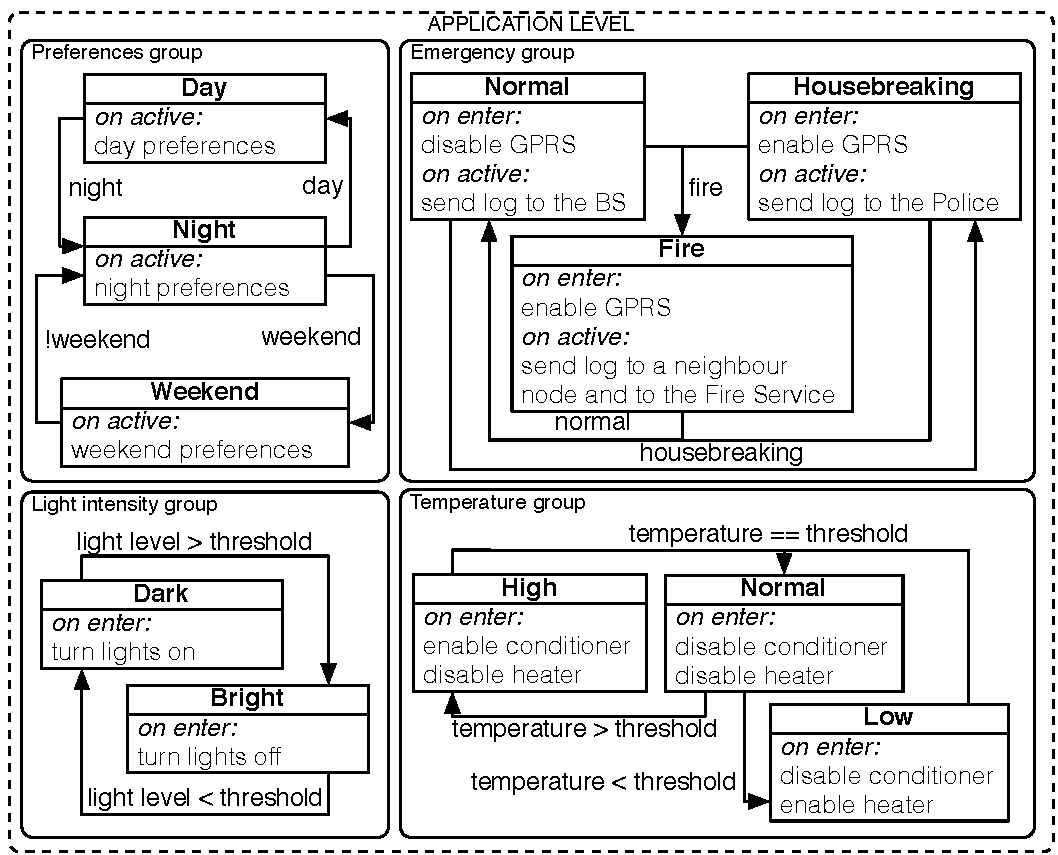
\includegraphics[width=\columnwidth]{pdf/smarthome}
}

The adaptive protocol stack, whose detailed context diagram we omit
for brevity, implements a dynamic protocol switching functionality in
situations where a node may alternative periods of significant
mobility to periods of static operation. The node roams within a
network of static nodes running CTP~\cite{CTP}. As long as the node
remains static, it joins the existing routing tree by running an
instance of CTP limited to being a leaf. As soon as the on-board
accelerometer detects a significant movement, it switches to a simpler
route-less gossip protocol~\cite{gossip}, which allows the node to
relay data to the static infrastructure
opportunistically~\cite{smarthop}. In addition, the node may switch
between three parameter sets for CTP, depending on context information
that determine whether lifetime, bandwidth, or XXXX\lm{Not sure what
  ``link quality adaptation means on the original diagram.} is to be
favored, similar to parameter adaptation in existing MAC protocols
depending on the presence of bursty traffic~\cite{contikiMAC,XMAC}.

% Another scenario - a system-level adaptation - is shown on Fig.~\ref{fig:apd}.
% If the network is static, it is feasible to use a \emph{Collection Tree
% Protocol}. In mobile network, however, a \emph{Gossip}-based protocol shows
% better results. Orthogonally to the \emph{Protocol type}, developer may want to
% adjust the \emph{Protocol parameters} to enhance a link quality between nodes,
% increase the lifetime of the network or use the bandwidth more effectively.

% \putfigure{caption=Adaptive protocol diagram.,label=fig:apd}{
%  \centering
%  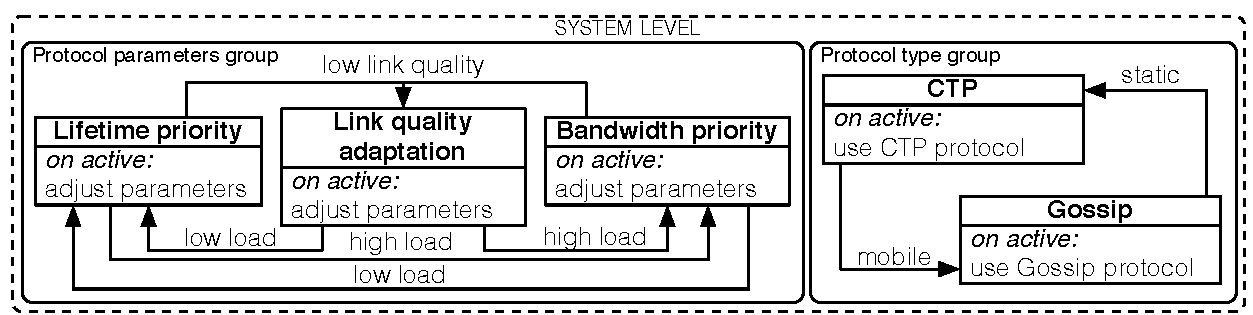
\includegraphics[width=\columnwidth]{pdf/system-level}
% }

\subsection{Coupling}\label{sec:evalcomp}

\begin{table}[!tb]
\renewcommand{\arraystretch}{1.3}
\caption{Coupling types.}
\label{tab:couptypes}
\centering
\begin{tabular}{|l|p{2.5in}|}
\hline
\bfseries Type & \bfseries Description\\
\hline
Content (tightest) & One module relies on the internal working of another. Chang- ing one module requires changes in the other as well.\\
\hline
Common & Two or more modules share some global state, e.g., a variable.\\
\hline
External & Two or more modules share a common data format.\\
\hline
Control & One module controls the flow of another, e.g., passing infor- mation that determine how to execute.\\
\hline
Stamp & Two or more modules share a common data format, but each of them uses a different part with no overlapping.\\
\hline
Data & Two or more modules share data through a typed interface, e.g., a function call.\\
\hline
Message (loosest) & Two or more modules share data through an untyped inter- face, e.g., via message passing.\\
\hline
\end{tabular}
\end{table}

According to Stevens et al.~\cite{stevens79}, seven types of coupling
between software modules exist, as summarized in
Table~\ref{tab:couptypes}. It is generally known that the tightest is
coupling, the more difficult is debugging, maintaining, and extending
the implementations. % Coupling types, which
% are presented in this section, are not forbidden in ConesC, but some
% of them can be easily avoided with a proper use of its concepts.
We investigate the types of coupling in \conesc and the nesC
implementations.

\begin{table}[!tb]
\renewcommand{\arraystretch}{1.3}
\caption{Coupling comparison: \emph{\conesc implementations save most types of coupling that are unavoidable in nesC.}}
\label{tab:coupres}
\centering
\begin{tabular}{|l|l|l|l|l|l|l|l|}
\hline
\bfseries Application & \rotatebox{90}{\bfseries Content} & \rotatebox{90}{\bfseries Common} 
& \rotatebox{90}{\bfseries External} & \rotatebox{90}{\bfseries Control}
& \rotatebox{90}{\bfseries Stamp} & \rotatebox{90}{\bfseries Data}
& \rotatebox{90}{\bfseries Message}\\
\hline
\hline
Wildlife tracking -- nesC &
yes&yes&yes&yes&--&yes&--\\
\hline
Wildlife tracking -- ConesC &
--&--&yes&--&--&yes&--\\
\hline
\hline
Smart-home -- nesC &
yes&yes&yes&yes&--&yes&--\\
\hline
Smart-home -- ConesC &
--&--&yes&--&--&yes&--\\
\hline
\end{tabular}
\end{table}

\fakepar{Results} Table~\ref{tab:coupres}\lm{Can we also count how
  many times we encounter a given type of coupling in either
  implementation?} illustrates the results of our analysis. Generally,
the ConesC implementations are significantly more decoupled compared
to their nesC counterparts.

Specifically, \conesc avoids \emph{Content} coupling in that different
behavioral variations are cleanly encapsulated in different
contexts. NesC programmers, on the other hand, cannot dynamically bind
command calls or event signals to different modules, which forces them
to expose internal module information that make one module's operation
depending on that of several others'. For the same reason, nesC
programmers are forced to use global state to switch between different
functionality depending on the situation. Such global state, which
creates \emph{Common} coupling, is not needed using \conesc, in that
the necessary functionality is automatically generated by our
translator. Finally, \conesc spares \emph{Control} coupling as
well. In essence, this comes as a result of allowing, in a sense,
dynamic binding across modules driven by the context transitions. Such
functionality, which is not available in nesC, needs to be hand-coded
in the latter.\lm{There was no explicit explanation for Common and
  Control... They were not mentioned.}


% Implementation of context components in ConesC, example of which are presented in Fig.~\ref{fig:cc} and~\ref{fig:irc}, do not rely on internal work of each other, so the are not coupled in the sense of~\emph{Content coupling}, as compared to nesC-written application, where all the behavioral variations are encapsulated in one module or function. Since each context represents a separate state of the environment or the device the system operates in, contexts are not intended to share any global states, to control the flow of each other and to pass the information how to execute. Our abstraction toward~\emph{context
% groups} allows developers to perform system-level operations -- e.g. data storage --
% orthogonally to the data processing without actual modules coupling involved.


However, both \conesc and nesC implementations show~\emph{Data}
and~\emph{External} couplings. This is unavoidable, in that different
modules in both implementations must necessarily agree on a common
data format and the C-based nature of nesC favors the use of typed
interfaces to rely on compiler-time type checking.
% We did not use, however, neither messages to share data
% nor different parts of the same data format, so~\emph{Stamp}
% and~\emph{Message} couplings are avoided in both implementations.


\subsection{Complexity}\label{sec:complexity}

We estimate the complexity of the implementations by measuring the
number of variable declarations and the number of functions in every
module. These are generally considered as intuitive indicators of a
program's complexity~\cite{pressman01}. It is also observed that
complexity is a function of the number of states in which the program
can find itself~\cite{35}. A state here is any possible assignment of
values to the program variables. Thus, the number of states must be
computed by looking at the different combinations of values assumed by
variables during every possible execution.

To carry out the latter analysis, we use SATABS~\cite{satabs}, a
model-checking tool for C programs already employed in sensor network
programming for similar analysis~\cite{mottola11survey}. SATABS is
designed for off-line verification of C programs against user-provided
assertions. To do so, it searches through the relevant program
executions to check whether the assertion always holds. At the end of
the process, SATABS returns the number of different states it explores
in the program.  Using a specific configuration, it is possible to
force SATABS to explore \emph{all} program executions. If the
procedure terminates, SATABS returns the total number of distinct
states of the program. We use SATABS on a per-function basis,
implementing empty stubs to replace code that we cannot process with
SATABS, e.g., hardware drivers.

\begin{table}[!tb]
\renewcommand{\arraystretch}{1.3}
\caption{Complexity comparison: \emph{\conesc yields simpler implementations that are easier to debug and to reason about.}}
\label{tab:compres}
\centering
\begin{tabular}{|l|c|c|c|c|c|c|}
\hline
&&&& \multicolumn{3}{@{\hspace{0.3em}}c@{\hspace{0.3em}}|}
{\bfseries Average per-module}\\[0.1in]
\bfseries Application & \rotatebox{90}{\bfseries LOC} 
& \rotatebox{90}{\pbox{0in}{\bfseries Variable\\declarations}} 
& \rotatebox{90}{\bfseries Functions} & \rotatebox{90}{\bfseries LOC}
& \rotatebox{90}{\pbox{0in}{\bfseries Variable\\declarations}}
& \rotatebox{90}{\bfseries Functions}\\
\hline
\hline
Wildlife tracking -- nesC&456&17&19&48&6&8\\
\hline
Wildlife tracking -- ConesC&539(440)&17&30&26,5&3&2\\
\hline
Wildlife tracking -- generated&1628&--&--&--&--&--\\
\hline
\hline
Smart-home -- nesC&360&24&28&28&2&2\\
\hline
Smart-home -- ConesC&382(289)&24&56&13&0,8&1,9\\
\hline
Smart-home -- generated&1310&--&--&--&--&--\\
\hline
\hline
Adaptive protocol -- nesC&150&10&13&38&2,5&3,25\\
\hline
Adaptive protocol -- ConesC&191(147)&5&21&14,7&0,4&1,6\\
\hline
Adaptive protocol -- generated&636&--&--&--&--&--\\
\hline
\end{tabular}
\end{table}

\fakepar{Results} Table~\ref{tab:compres} illustrates our
results\lm{Now that we have good results for the number of states, I
  think we can avoid discussing the implementation-wise numbers and
  LOC.}. On a per-module basis, \conesc shows significant reductions
in both the number of declared variables and defined functions. This
comes from the ability to dynamically bind a function call to the
required context-dependent implementation transparently to the
caller. In nesC, on the other hand, this requires defining global
variables to check what behavior needs to be triggered as a function
of the current situation. As a result of this, the number of
per-function states programmers must manage also decreases
drastically, making the implementations simpler to
understand. Together with the concepts of \emph{contexts}
and~\emph{context groups}, which help in better organizing the code,
this facilitates debugging and maintenance.

%  -- and
% boilerplate code. Because of the same reason, functions have to be
% spitted into smaller isolated parts. We believe, however, that in
% larger applications the number of the similar lines of code will be
% bigger.  

% The number of LOC can also be decreased significantly -- as
% shown in Table~\ref{tab:compres} in parentheses -- by having a tool,
% which generates a boilerplate code using a diagram of a
% context-oriented model of the application, similar to the one
% displayed in Fig.~\ref{fig:wtd}. The logical fragmentation leads to a
% code simplification, improved readability and re-useability along with
% easier debugging and maintaining processes.

As debatable as it may be for measuring the effectiveness of a
programming abstraction~\cite{mottolasurvey}, we also measured the
number of lines of code in both nesC and \conesc implementations. The
two are roughly comparable. More interestingly, we also measured the
size of the code generated by our translator, described in
Section~\ref{sec:translator}, as a measure of the expressive power of
\conesc, that is, the amount of processing that \conesc programmers
can succinctly express using the abstractions we design. It turns out
that the output of our translator is roughly \emph{three times} the
size of the input code, intuitively demonstrating that our
abstractions do capture a significant portion of processing in a few
simple concepts.


% as shown on Table~\ref{tab:compres}, we notice that the
% program written in context-oriented style using plane nesC is more
% than 3 times bigger than its ConesC counterpart. Our approach makes
% context-oriented programming as simple as plain nesC programming.

\subsection{MCU and memory overhead}\label{sec:overhead}

The advantages brought to programmers come at the cost of additional
system overhead. To assess this, we measure the MCU overhead for
context transitions and calls to layered functions, as well as memory
overhead when using \conesc as compared to nesC. To measure the MCU
overhead we use the MSPSim MSP430 emulator~\cite{eriksson09}, while we
estimate the memory overhead using the tools in the nesC and GNU-C
toolchains.

% Since there are neither contexts nor layered functions in nesC-based
% implementation, we measured a number of CPU-cycles of parts with different
% execution flow. For example, contextual events, like a base station presence,
% are detected and handled in ConesC differently as compared to nesC, but,
% eventually, it results in the same functionality. 

\fakepar{Results} Fig.~\ref{fig:cmo}\lm{We should change ``protocol''
  to''stack'' in the picture.} shows the results. The average MCU
overhead for a layered function call ranges from 2 to 5 MCU cycles,
depending on the application. Such figures are negligible in terms of
energy consumption, since the simplest operation in TinyOS, that is
turning on/off an LED, already consumes 8 MCU cycles. The overhead of
context transitions is slightly larger, but in the same order of
magnitude. Most importantly, the memory overhead is also negligible,
measuring a worst-case 2.5\% penalty for the size of the program
binary and a worst-case 4.5\% penalty for RAM usage.\lm{Do we have an
  explanation as to why the adaptive protocol case is the smallest?}

\putfigure{caption=MCU and memory overhead: \emph{the resource usage penalty for using \conesc is almost negligible.},label=fig:cmo}{
\centering
\subfloat[MCU overhead.]{
  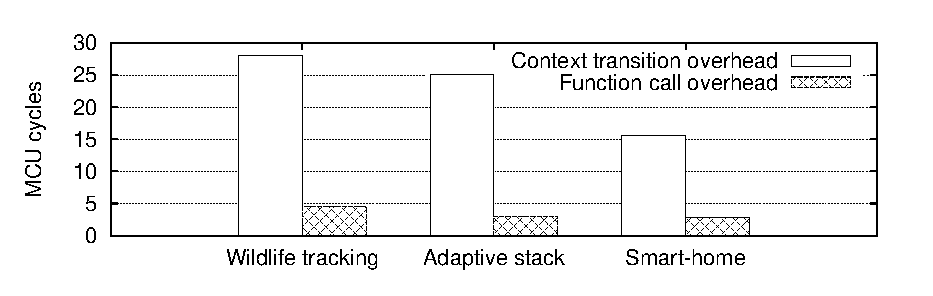
\includegraphics[width =0.5\columnwidth]{pdf/cpu_overhead}
  \label{fig:cpuo}
}
\subfloat[Memory overhead.]{
  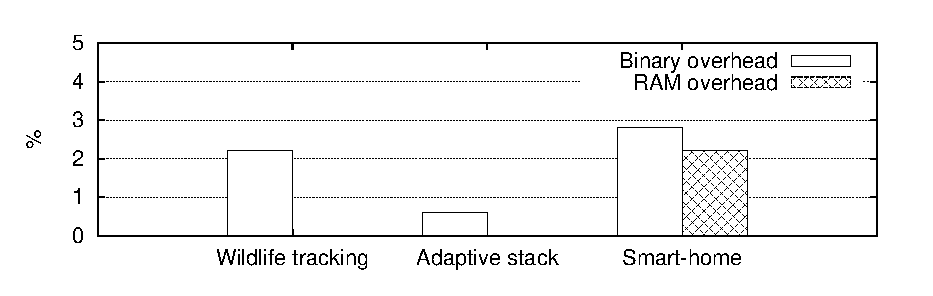
\includegraphics[width=0.5\columnwidth]{pdf/memory_overhead}
  \label{fig:memo}
}
}


%%% Local Variables: 
%%% mode: latex
%%% TeX-master: "bare_conf"
%%% End: 
